\chapter{Theoretical Part -- Data Processing}\label{ch:data_processing}
The goal of this thesis is to design a data processing pipeline with an appropriate storage system suitable for the described use case. This chapter will focus on the computational and data-processing part. It is assumed that the necessary storage solutions already exist, and only the theory of data processing will be discussed to build fundamental knowledge that will later be applied in the implementation.

The goal of this chapter is to introduce the fundamentals, serving as a starting point for any similar data processing system.

\section{Data Processing}
In the thesis, data processing refers to the process of moving and transforming selected binary data.

There are three distinct types of data processing systems that need to be distinguished. Each of these systems requires different solutions that are optimized and tuned to its needs.
\begin{itemize}
    \item \textbf{Online (service systems)} \\
    The online (service) data processing system is a request-based system in which data are processed per client request. Processing begins when the system receives a request, and the service must produce output to respond to the client. In such a system, the main criterion (to optimize for) is response time -- the latency between request and response, and parameter availability of the system. Those two are considered the most important in such a system.
    \item \textbf{Offline processing systems (batch systems)} \\
    The batch-processing (offline) system is typically used to process large amounts of input data at once. This type of processing is not focused on speed (since it may take from a few minutes to several days), but is optimized for throughput. Such processes are often run periodically and are scheduled as jobs. It is not focused on availability, but on quality and throughput.
    \item \textbf{Stream processing systems (near-real-time systems)} \\
    Stream processing lies between offline and online processing. Like in batch processing, it typically process a large amount of work and processes them in parallel; it also does not typically produce a response, but some output, which is later stored in any type, including a database, event, file, etc. \\
    On the other hand, it usually processes the data as soon as the event or job is available to the system. This is more similar to online processing.
\end{itemize}\cite{kleppmann_designing_2017}

This thesis focuses on stream processing systems (also known as near-real-time systems). Since stream processing combines online and offline processing, it needs to incorporate concepts from both. The method for combining both systems and building a streaming data pipeline system will be discussed in Section \ref{sec:pipeline_architectures} 

\section{Pipelines}
In modern software architecture, the mechanism responsible for moving and transforming data is called a data pipeline. It usually involves the transport of data, its validation, transformation, and management during transit. In the context of the thesis, the pipeline includes downloading images, processing them, deriving image metadata, storing data in internal storage, computing image embeddings, and outputting the embeddings. \cite{kleppmann_designing_2017}

A data pipeline is, in general, any automated process that runs a predefined sequence of operations. It begins with a clearly defined input, which can be the data itself or information on how to access the data. When data enter the pipeline, they are processed by a series of steps. Those steps can always be represented as an acyclic graph (DAG). At the end of the pipeline, it provides a clear data-processing output or stores it in the required systems. This makes the whole pipeline well-defined and clear, so it can be reproduced at any time for any amount of data. \cite{kleppmann_designing_2017}

In practical implementations, individual operations (part of the pipeline) are frequently aggregated into logical units called \textit{jobs}. They encapsulate a specific sequence of related tasks -- such as downloading, resizing, and saving.

\subsection{Job}\label{sec:job}
Units of operations in the pipeline are often referred to as jobs. Jobs are parts of a pipeline that can be logically isolated. Those parts are typically responsible for the subtasks of the pipeline, and by chaining them together, they form a whole (data) pipeline. Such parts can be understood as small programs (a list of instructions) that convert well-defined input to well-defined output (same as the whole pipeline). In a more abstract sense, jobs can be understood as smaller pipelines that together form a single larger pipeline.

The idea of jobs is an old concept in software engineering known as modularity. Modularity offers a new way to approach problems by breaking them into smaller pieces (rather than maintaining a single monolithic solution). Even though modularity is an old, intuitive concept, it has become more popular with the rise of distributed systems and microservice architectures.\cite{reis_fundamentals_2022}\footnote{As many think in modern computer science.}

Isolating a series of instructions in a pipeline into units called jobs allows more control over the input and output of each job, breaks tight coupling, and defines well-defined points throughout the pipeline. Such points can later be used for failure reporting, recovery, etc. Among other advantages, breaking pipelines into loosely coupled chunks allows better scalability and planning. \cite{reis_fundamentals_2022}

\subsection{Pipeline -- Chaining Jobs}
As defined in Section \ref{sec:job}, a job represents a single logical unit of work. However, complex data processing tasks rarely consist of a single job. Instead, they require the sequential or parallel execution of multiple distinct steps (jobs). This composition of jobs is referred to as \textit{chaining}, and the resulting structure forms the \textit{data pipeline}.

By chaining jobs, the pipeline acts as a layer that manages the flow of data from one unit to the next. This architecture offers several advantages over monolithic data processing scripts.

\subsubsection*{Fault Tolerance and Recovery}
One benefit of breaking a pipeline into units is improved recovery when execution fails. In a monolithic process, each error must be handled separately, and recovery usually requires restarting the entire process from the beginning. In a chained pipeline, errors must be handled the same way as in monolithic code, but each job can serve as a checkpoint, allowing recovery. 

If a specific job fails, the system can identify exactly which step encountered an error. Because the state of the data is defined at the input and output of every job, the pipeline can often be restored, starting only from the failed job, rather than re-starting the entire process. This \textit{unit of failure} approach significantly reduces the cost of errors and simplifies debugging.

\subsubsection*{Modularity and Replaceability}
Decomposing a complex pipeline into a chain of jobs enforces modularity. Since each job is a unit with a strictly defined input and output, individual jobs can be updated, optimized, or entirely replaced without affecting the rest of the pipeline.

For example, a specific image resizing algorithm in the middle of a pipeline could be swapped for a more efficient library. As long as the input/output interface remains consistent, the surrounding jobs (downloading or storing) remain unchanged. This decoupling enables easier maintenance and iterative system improvement.

\subsubsection*{Scalability and Distributed Execution}
Pipeline architecture is, by design, suitable for distributed computing. Because jobs are isolated, they do not necessarily need to run on the same physical machine. A pipeline orchestrator can distribute different jobs across multiple nodes in a cluster.

This enables horizontal scaling: if the image embedding job is computationally intensive and limits throughput, it can be scaled out to run across multiple worker nodes in parallel, while lighter jobs (such as metadata extraction) run on fewer resources. This flexibility allows the system to maximize resource utilization and throughput.

The dependencies between jobs naturally form a Directed Acyclic Graph (DAG). By explicitly defining which jobs depend on the output of others, the system can identify pipeline branches that are independent of one another. These independent branches can be executed in parallel across different nodes, significantly reducing the total processing time. \cite{kleppmann_designing_2017}

\section{Pipelines for Data Processing Systems}\label{sec:pipeline_architectures}
As discussed in the previous Section \ref{ch:data_processing}, data processing systems can be categorized into three distinct types: online (service) systems, offline (batch) systems, and stream processing systems. In the introduction to this thesis, it was established that the primary goal is to design and implement a stream processing pipeline.

Since stream processing is conceptually a hybrid of online and offline processing, it inherits characteristics from both. The following section will describe online, offline, and lastly stream solutions, which will often be a combination of both approaches. The text will discuss 4 components that need to be designed for such pipelines: input, connector, worker, and output. To better understand these architectural designs, refer to Figures \ref{fig:online-pipeline}, \ref{fig:offline-pipeline}, \ref{fig:stream-pipeline} during reading.

All architectural designs come from different needs, and ways of data processing like specified above.

\subsection{Data Input and Triggering}
The first fundamental difference between the architectures is how data enter the system and what triggers the processing.

\begin{itemize}
    \item \textbf{Online:} In online systems, input is typically handled via standard network protocols such as REST (HTTP) or gRPC. The trigger is external (a request), and processing begins immediately upon receipt of a request. Requests are typically sent by the user or other systems, which use the pipeline.
    \item \textbf{Offline:} Offline systems do not respond to any external request; they rely on a scheduled or manual trigger. The input is usually a bounded set of data (work) available in some form (typically storage). The process is initiated by a human operator or a time-based scheduler (e.g., CRON) once all required data are collected and the necessary resources to run the pipeline are available.
    \item \textbf{Stream:} Stream pipelines process data that arrive in the system without knowing when it happens and at what load, typically using an event-driven input model. To handle input, the use of a queue or an event log to hold processing requests for the pipeline is required. Processing is triggered by the arrival of an event. As soon as data are pushed to the queue, the pipeline consumes it, combining the automated nature of online systems with the decoupling of offline systems. Such an architecture allows the system to react to incoming messages almost immediately (near real-time) and still handle large loads of data to be processed by keeping requests in a job queue.

\cite{kleppmann_designing_2017, reis_fundamentals_2022}
\end{itemize}

% refrazed
\subsection{Connectors and Transport}
Transporting data between different stages (jobs) of a pipeline requires different solutions for each type of data processing system. Solutions influence the capacity, latency, and durability of stage connectors (which hold the state of processed data).

\begin{itemize}
    \item \textbf{Online:} Communication is primarily handled via the network. A network enables minimizing latency, which is needed for online processing. A downside of using the network is the inability to recover from failures at any stage of the pipeline, since data are not persistent. This is typically not a problem since the user can receive an error response and a repeat request if needed. \\
    Services typically communicate synchronously over the network, expecting an immediate reaction.
    \item \textbf{Offline:} The primary connector is \textit{storage}. One stage of a job writes data to a storage or database, and the next stage reads from that storage. The storage acts as the interface between steps. This allows recovery from any stage where an error may have occurred. Introducing storage may introduce additional latency. This should not be a common issue, as offline processing typically runs for extended periods and the latency is not significant across the entire process.
    \item \textbf{Stream:} To handle continuous flow and potential pressure, stream systems typically use \textit{Message Queues} (or Message Brokers). The queue acts as a buffer, ensuring that data are not lost if processing requests spike and the pipeline is not scaled to handle such a load.

\cite{kleppmann_designing_2017}
\end{itemize}

% refrazed
\subsection{Resource Allocation}
The strategy for resource allocation and worker lifecycle differs significantly based on the expected load pattern.

\begin{itemize}
    \item \textbf{Online:} Jobs must always be running and available to serve responce with as low latency as possible. Even during idle periods, resources are reserved to ensure immediate response capability when a request arrives. Such solutions are resource-intensive because they have to keep running workers to handle the largest expected load.
    \item \textbf{Offline:} Workers are ephemeral. During idle times, zero workers are running. When a job is triggered, the system spawns as many workers as the hardware resources or parallelization logic allow, runs them at full capacity, and terminates them upon completion. Sections in pipelines are typically allocated to each job independently to achieve high throughput. This is possible because the data state between stages is stored permanently.
    \item \textbf{Stream:} Stream processing uses scalable workers. While the system requires a baseline number of running workers to ensure availability (as in online systems), it must scale dynamically during peak traffic to maintain throughput. This ensures resource efficiency -- scaling up during high load and scaling down (but not to zero) during low load.
\end{itemize}

\subsection{Output and Results}
Finally, the systems differ in what they produce as a result of the processing.

\begin{itemize}
    \item \textbf{Online:} The output is a response to the user or the system. The system must return data or a confirmation status back to the client that initiated the request.
    \item \textbf{Offline:} The output is typically a report or a transformed dataset stored in a database/storage. There is no direct client waiting for a response.
    \item \textbf{Stream:} Stream pipelines often produce both. They generate reports (aggregated data stored for analysis) and can also trigger responses or side effects (such as alerts or push notifications) in real-time.
    
\cite{kleppmann_designing_2017}
\end{itemize}

\begin{figure}[h!t]
    \centering
    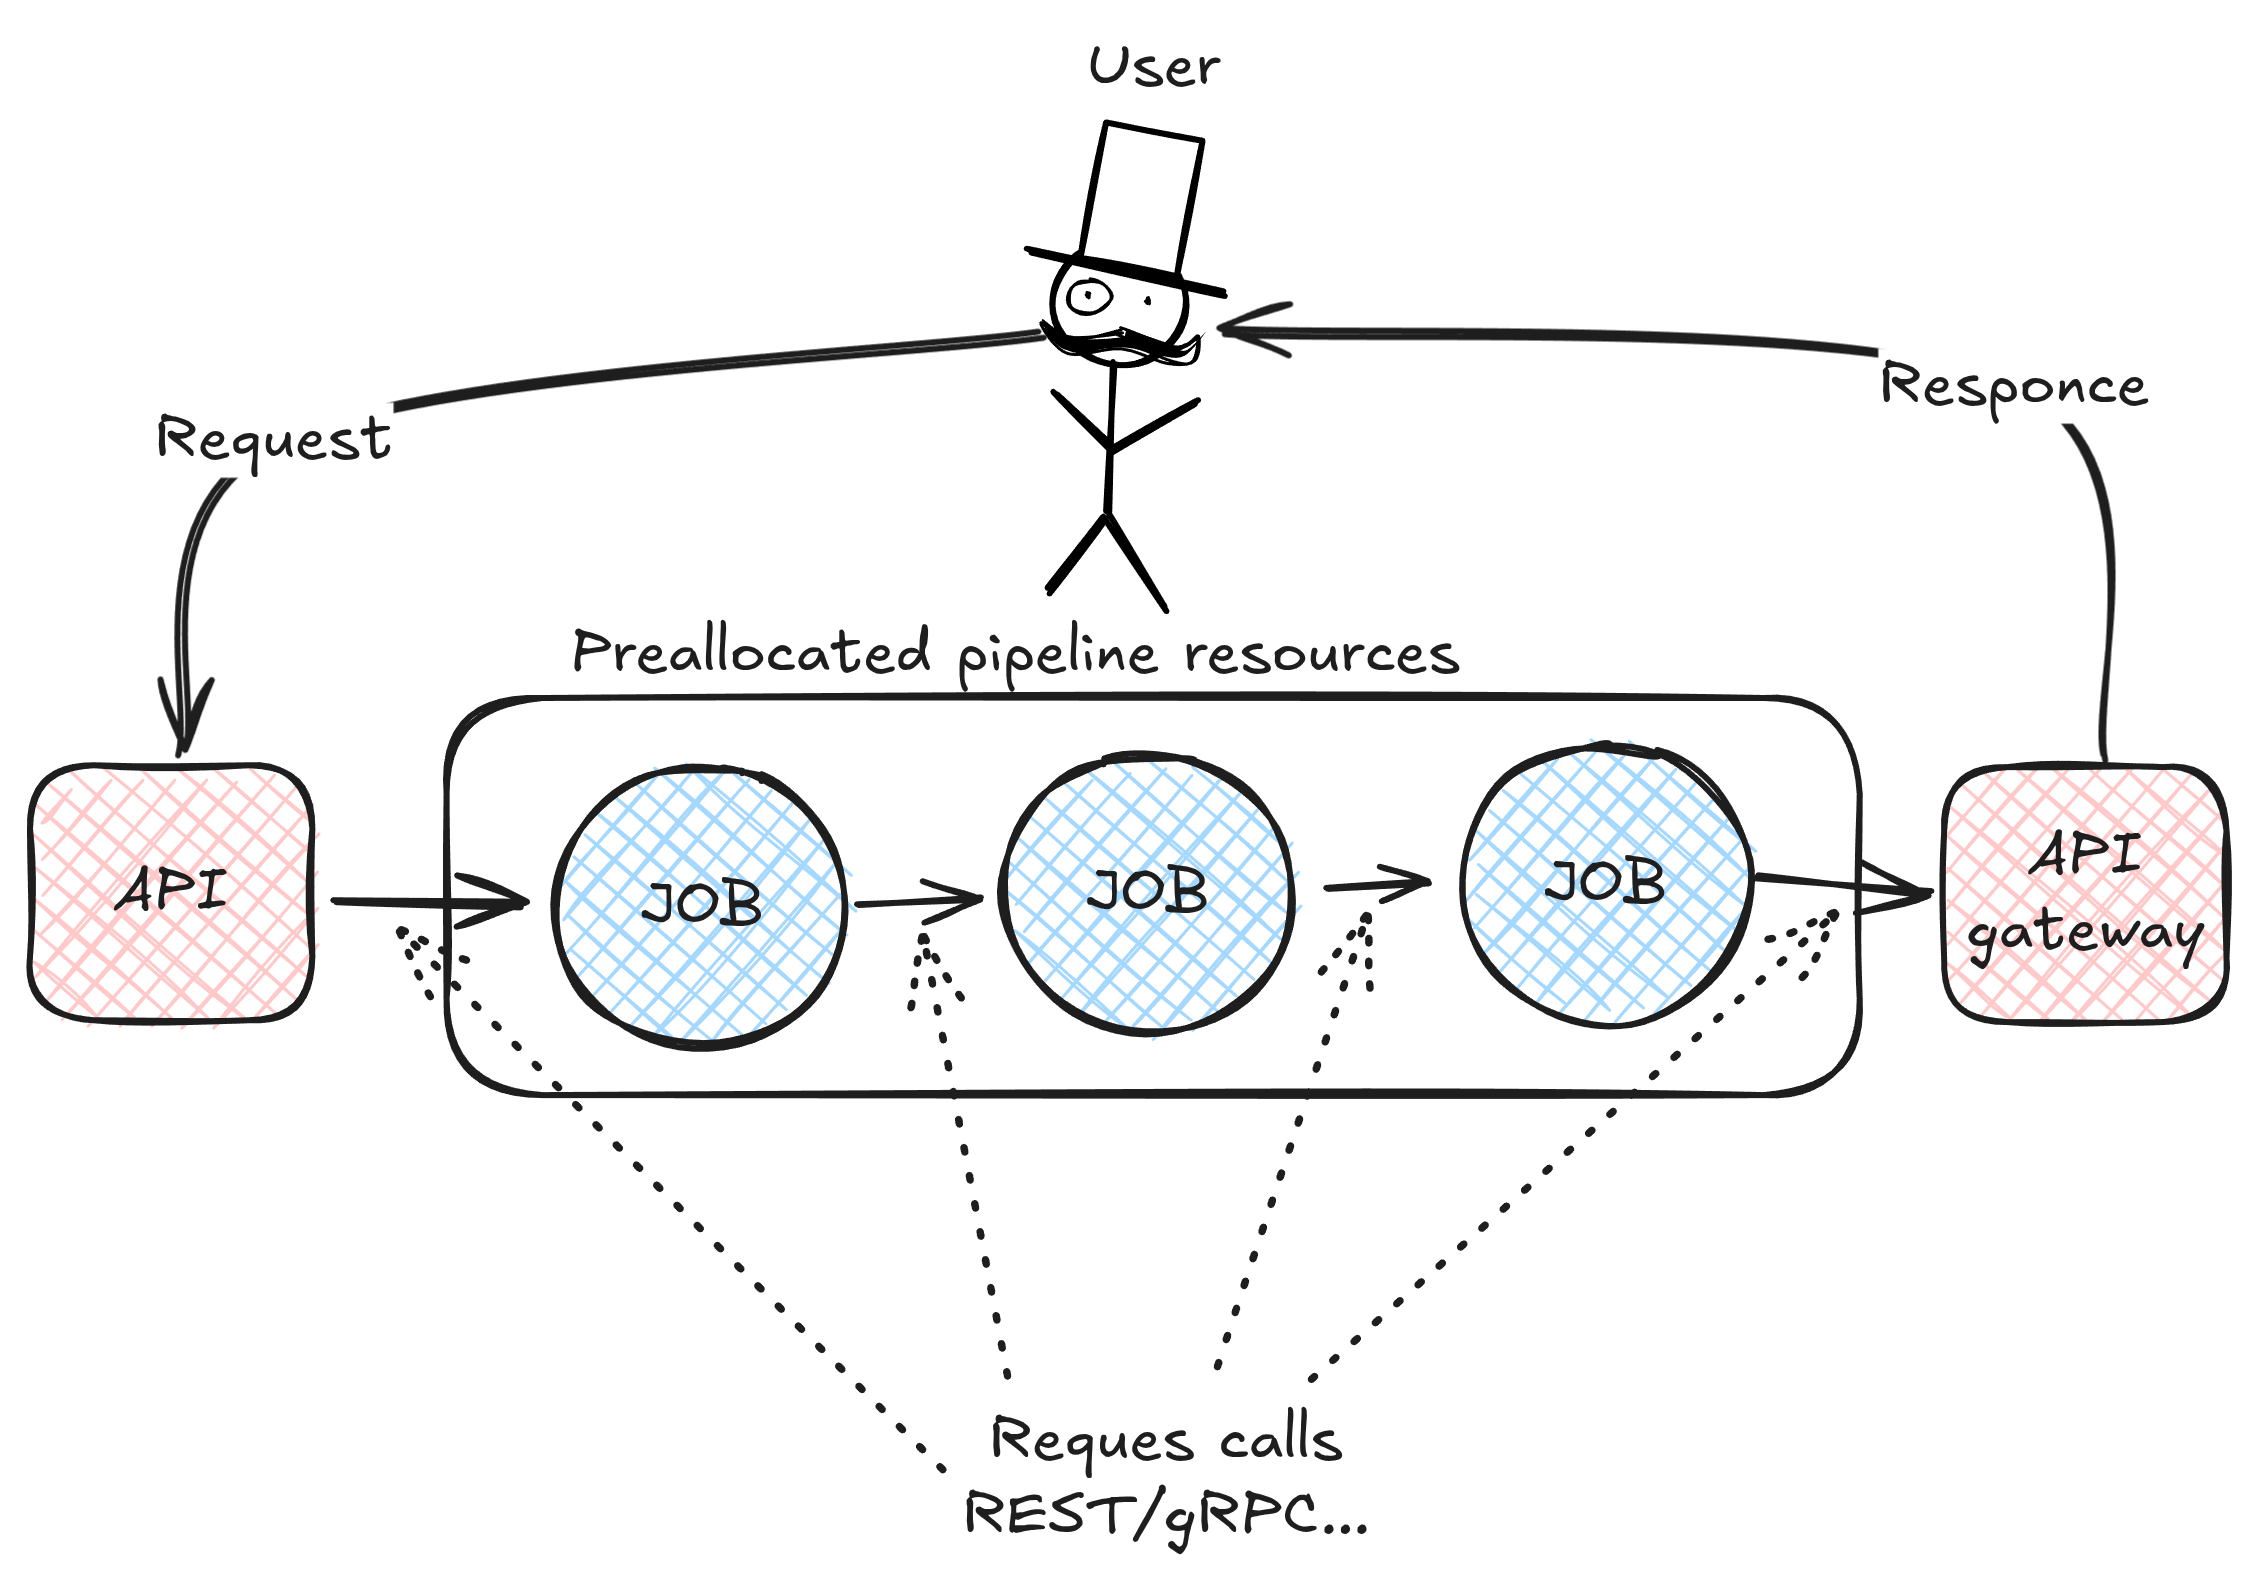
\includegraphics[width=0.8\textwidth]{images/online-pipeline.png}
    \caption{\label{fig:online-pipeline}Online pipeline}
\end{figure}

\begin{figure}[h!t]
    \centering
    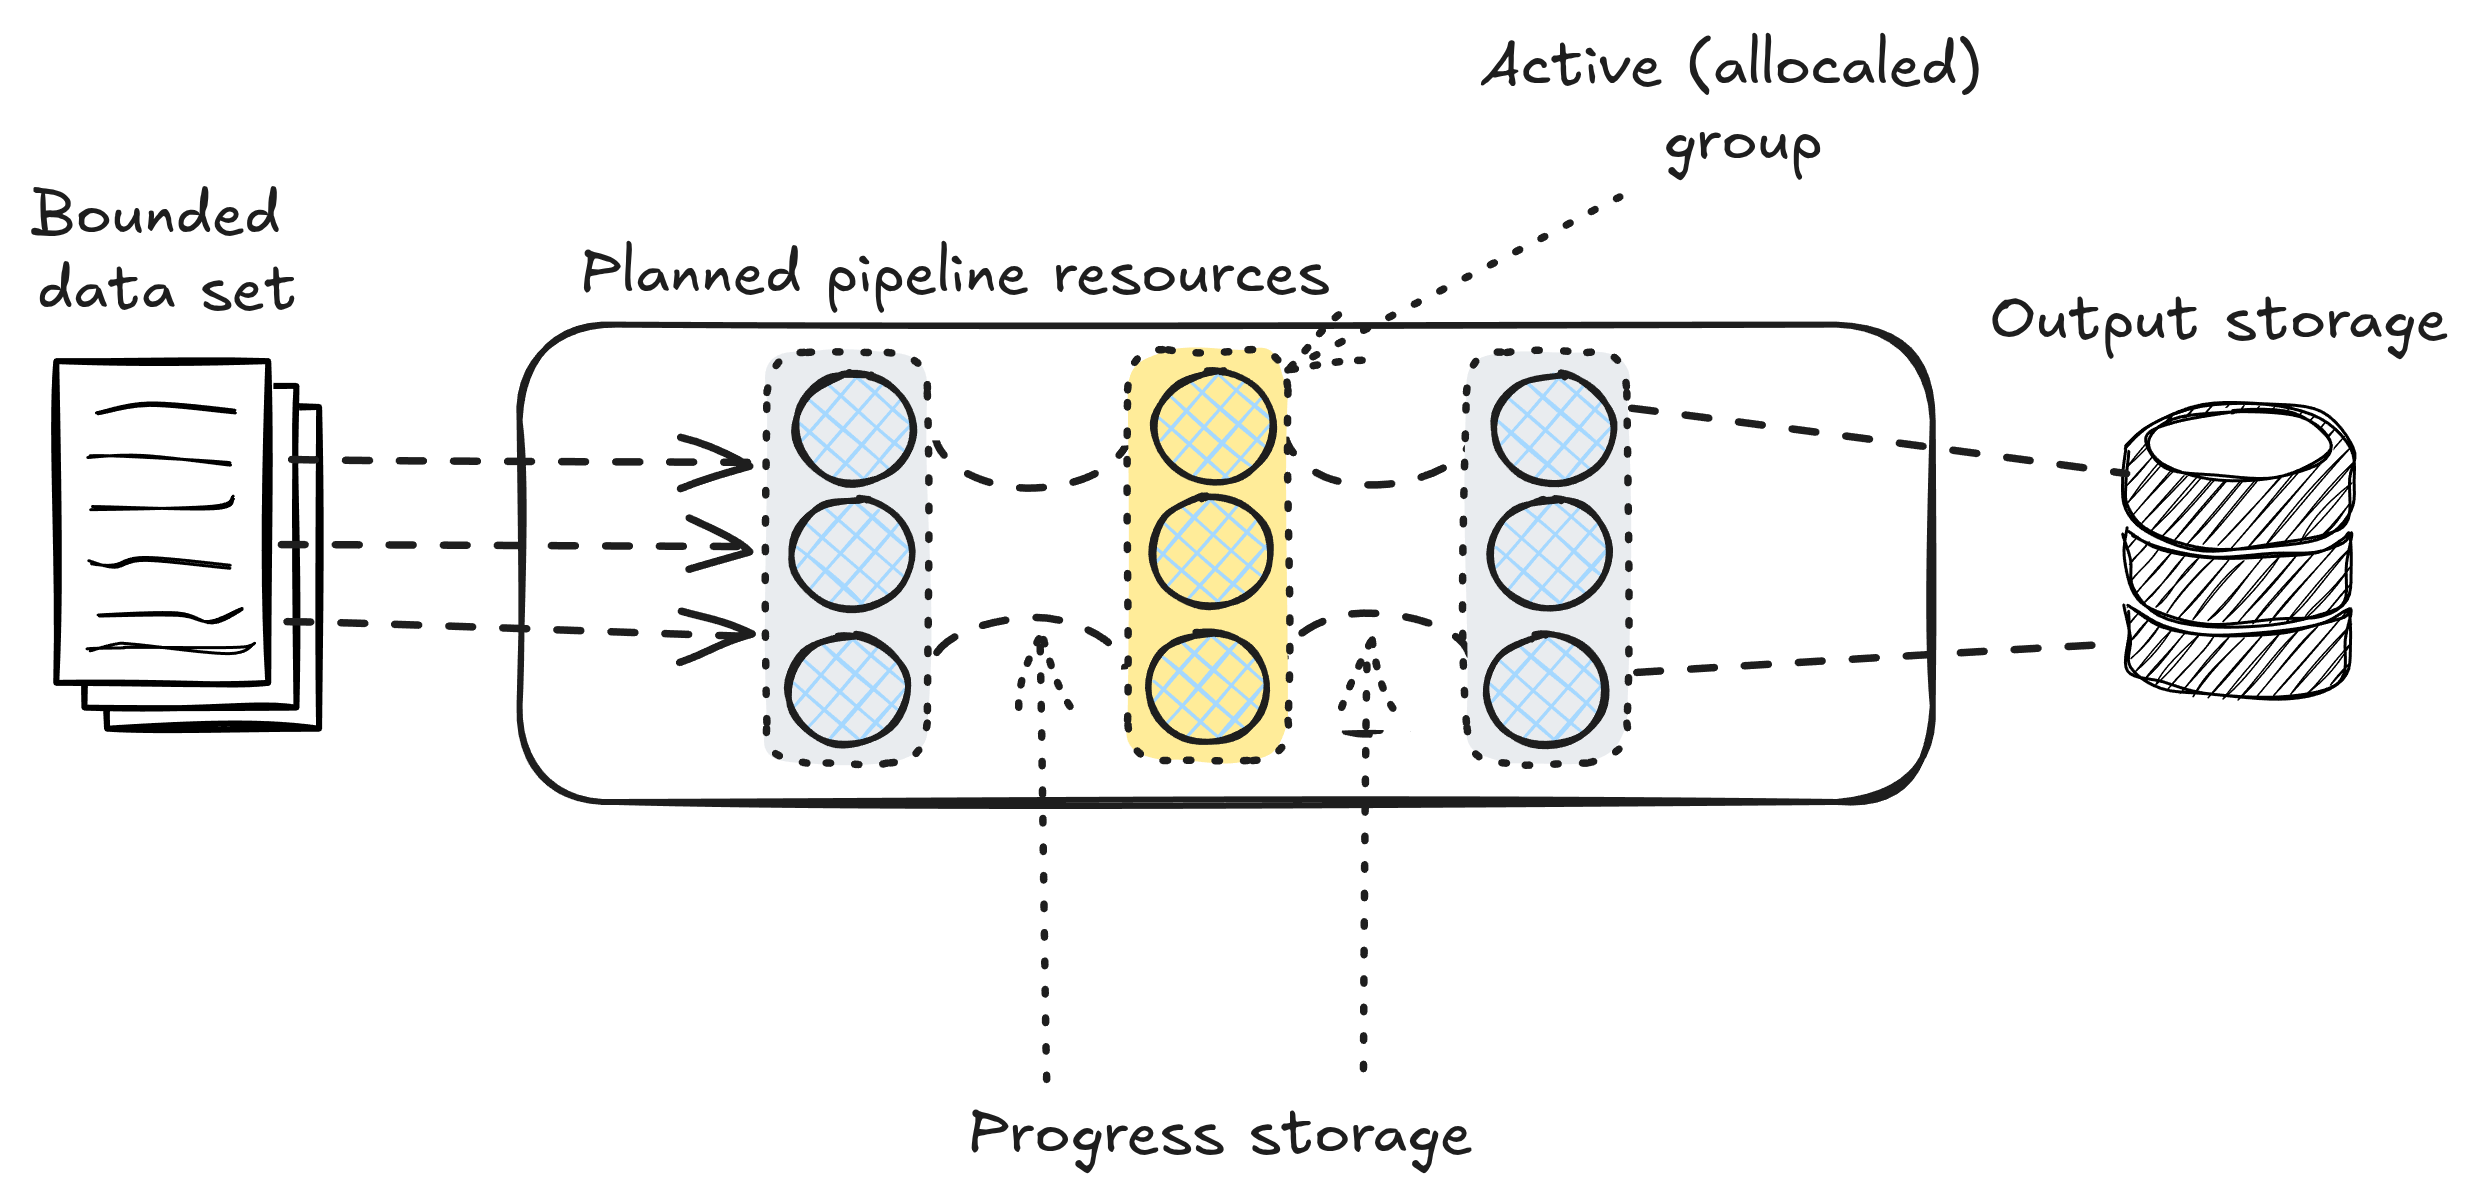
\includegraphics[width=0.8\textwidth]{images/offline-pipeline.png}
    \caption{\label{fig:offline-pipeline}Offline pipeline}
\end{figure}

\begin{figure}[h!t]
    \centering
    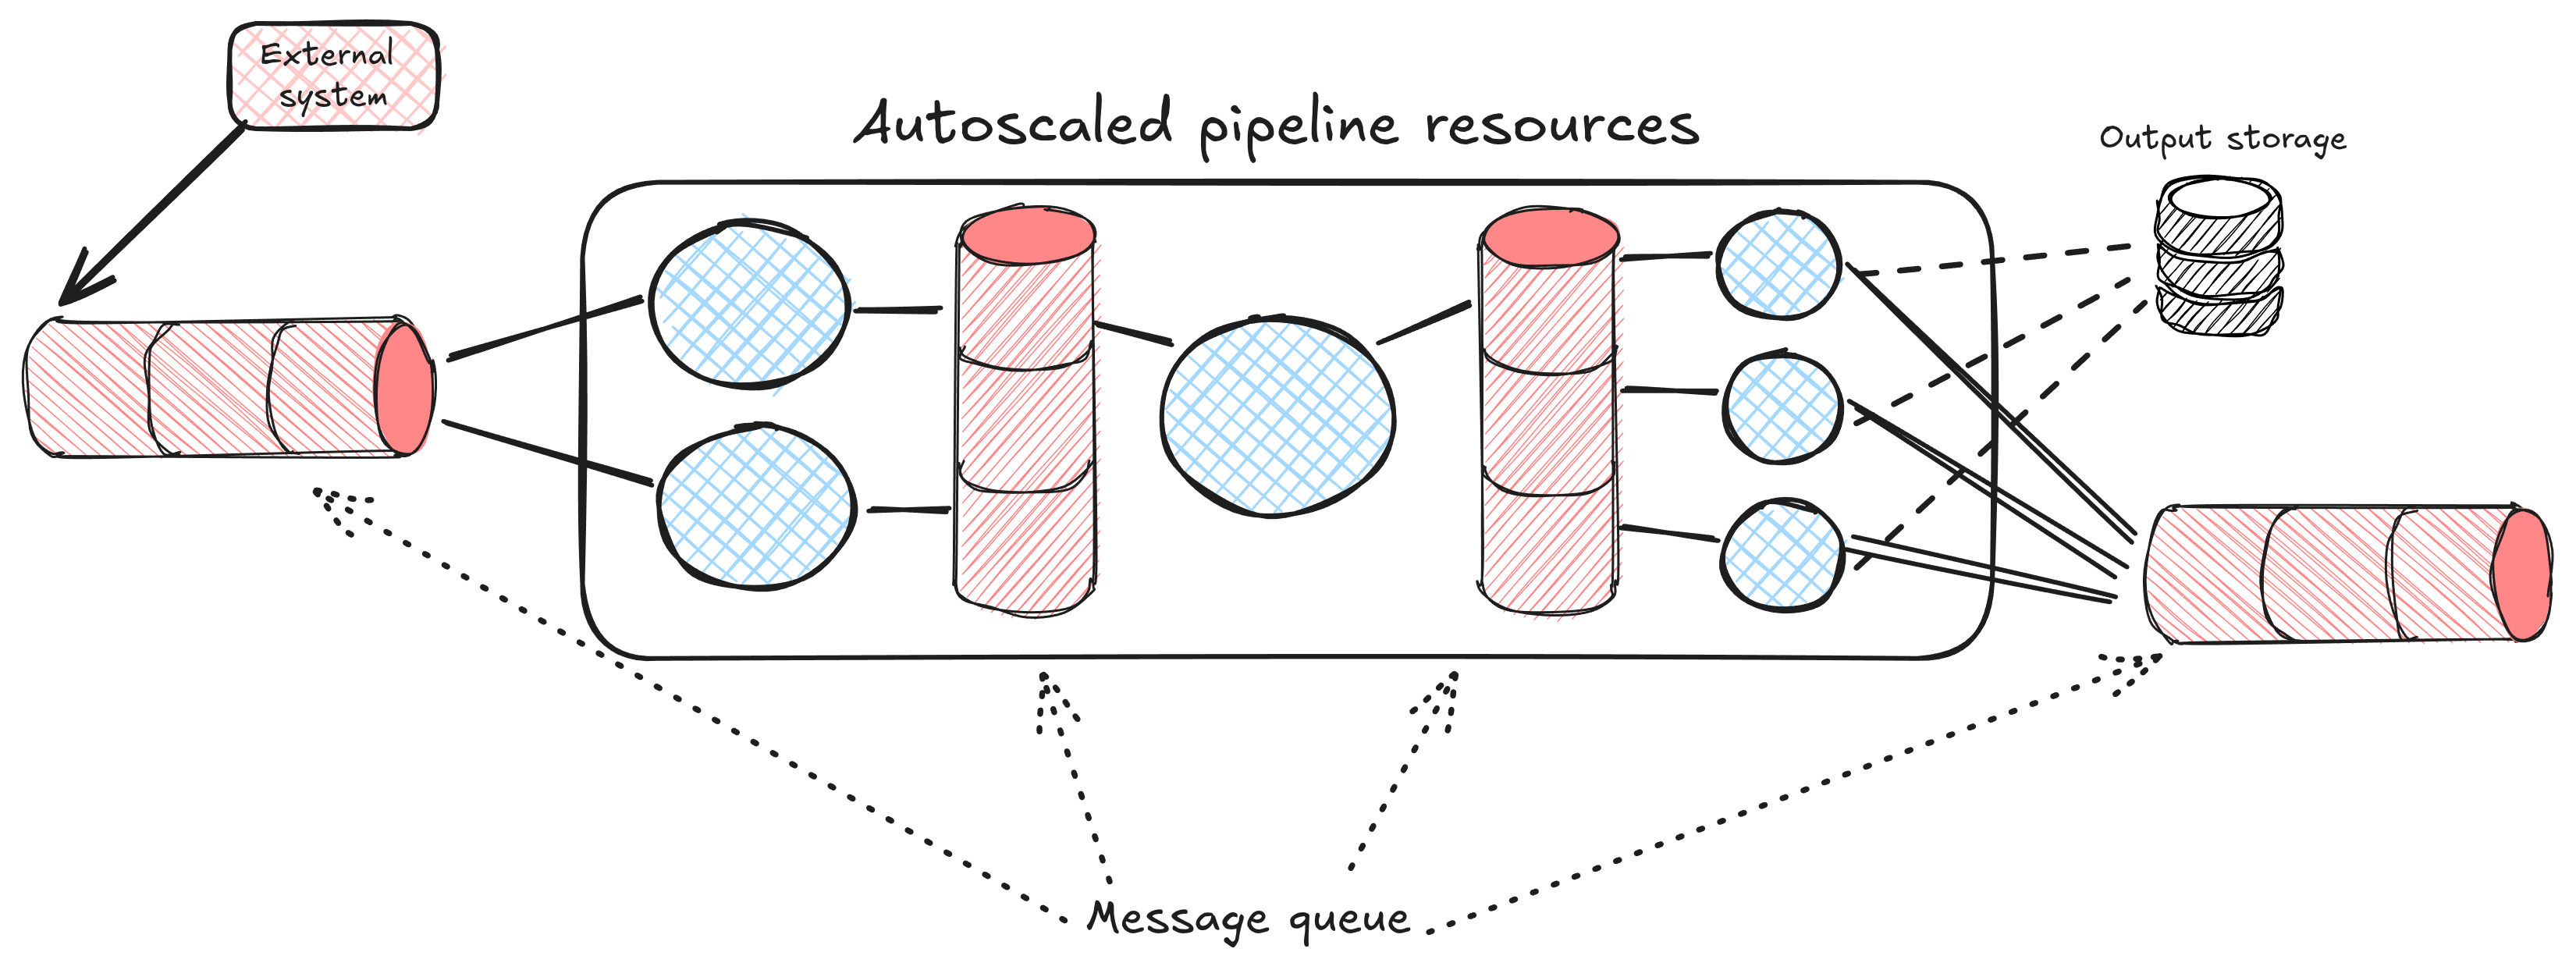
\includegraphics[width=0.8\textwidth]{images/stream-pipeline.png}
    \caption{\label{fig:stream-pipeline}Stream pipeline}
\end{figure}
